\documentclass[fleqn]{article}
\usepackage[utf8]{inputenc}
\usepackage[spanish, es-lcroman]{babel}
\usepackage[margin = 15mm]{geometry}
\usepackage{parskip}
\usepackage{amsmath, amssymb, amsfonts}
\usepackage{enumerate}
\usepackage{graphicx}

\expandafter\def\expandafter\normalsize\expandafter{%
    \setlength\abovedisplayskip{-9pt}%
    \setlength\belowdisplayskip{5pt}%
}

%\renewcommand{\theenumi}{\roman{enumi}}

\newcommand{\real}{\mathbb{R}}
\newcommand{\ent}{\mathbb{Z}}
\newcommand{\intg}[3]{\int_{#1}^{#2} #3 \, \mathrm{d}x}

\begin{document}
	\bfseries
	Ecuaciones Diferenciables Parciales \\
	Tarea 4 \\
	Osmar Dominique Santana Reyes \\
	No. de cuenta: 2125197 \\

	\begin{enumerate}[I.]
		\item Construya la serie de Fourier completa de la función dada $f$. En cada caso, utilice esquemas apropiados y analice la convergencia de la serie en el intervalo $ [-L,L] $ donde $f$ está definida.
		
		\begin{enumerate}[(1)]
			\item $ f(x) = \begin{cases}
				-2, & -1 \leq x \leq 0 \\
				3, & 0 < x \leq 1 \\
			\end{cases} $

			Solución.

			\normalfont

			\begin{equation*}
				a_0 = \dfrac{1}{1} \intg{-1}{1}{f(x)} = \intg{-1}{0}{-2} + \intg{0}{1}{3} = -2 + 3 = 1
			\end{equation*}

			\begin{equation*}
				a_n = \dfrac{1}{1} \intg{-1}{1}{f(x) \cos \left( \dfrac{n \pi x}{1} \right)} = \intg{-1}{0}{-2 \cos \left(n \pi x \right)} + \intg{0}{1}{3 \cos \left(n \pi x \right)} = 0
			\end{equation*}

			\begin{align*}
				b_n &= \dfrac{1}{1} \intg{-1}{1}{f(x) \sen \left( \dfrac{n \pi x}{1} \right)} = \intg{-1}{0}{-2 \sen \left(n \pi x \right)} + \intg{0}{1}{3 \sen \left(n \pi x \right)} \\
				&= \dfrac{2(1 - (-1)^n)}{n \pi} + \dfrac{3(-(-1)^n + 1)}{n \pi} = \dfrac{5(1 - (-1)^n)}{n \pi}
			\end{align*}

			Así, $ \displaystyle f(x) \sim \dfrac{1}{2} + \sum_{n=1}^{\infty} \dfrac{5(1 - (-1)^n)}{n \pi} \sen (n \pi x) $

			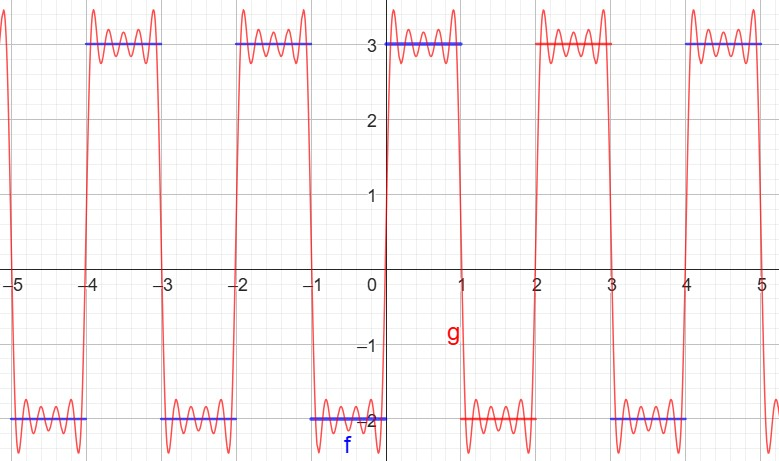
\includegraphics[width=\linewidth]{Ejer1.jpg}

			Luego, como $f$ es suave por tramos en $ [-1,1] $, se tiene que la serie de fourier de $f$ converge puntualmente a la extensión periódica de $f$ a $ \real $ en todo $ x \in \real \setminus \ent $ y a $ \dfrac{f(x^-) + f(x^+)}{2} = \dfrac{3-2}{2} = \dfrac{1}{2} $ en todo $ x \in \ent $.

			\bfseries 
			\item $ f(x) = \begin{cases}
				x, & -1 \leq x \leq 0 \\
				2x - 1, & 0 < x \leq 1 \\
			\end{cases} $

			Solución.

			\normalfont

			\begin{equation*}
				a_0 = \dfrac{1}{1} \intg{-1}{1}{f(x)} = \intg{-1}{0}{x} + \intg{0}{1}{2x - 1} = -\dfrac{1}{2}
			\end{equation*}

			\begin{align*}
				a_n &= \dfrac{1}{1} \intg{-1}{1}{f(x) \cos \left( \dfrac{n \pi x}{1} \right)} = \intg{-1}{0}{x \cos \left(n \pi x \right)} + \intg{0}{1}{(2x - 1) \cos \left(n \pi x \right)} \\
				&= \dfrac{1 - (-1)^n}{\pi^2 n^2} + \dfrac{2((-1)^n - 1)}{\pi^2 n^2} = \dfrac{(-1)^n - 1}{\pi^2 n^2} 
			\end{align*}

			\begin{align*}
				b_n &= \dfrac{1}{1} \intg{-1}{1}{f(x) \sen \left( \dfrac{n \pi x}{1} \right)} = \intg{-1}{0}{x \sen \left(n \pi x \right)} + \intg{0}{1}{(2x - 1) \sen \left(n \pi x \right)} \\
				&= -\dfrac{(-1)^n}{n \pi} - \dfrac{(-1)^n + 1}{n \pi} = - \dfrac{2(-1)^n + 1}{n \pi}
			\end{align*}

			Así, $ \displaystyle f(x) \sim -\dfrac{1}{4} + \dfrac{1}{\pi} \sum_{n=1}^{\infty} \left[ \dfrac{(-1)^n - 1}{\pi n^2} \cos (n \pi x) - \dfrac{2(-1)^n + 1}{n} \sen (n \pi x) \right] $

			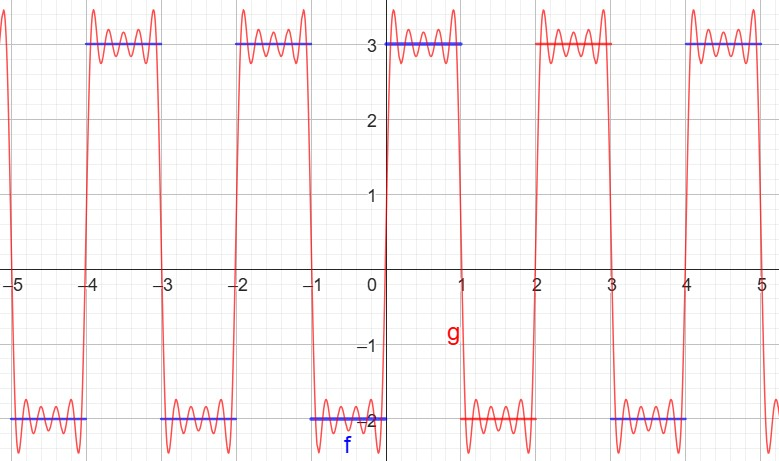
\includegraphics[width=\linewidth]{Ejer1.jpg}

			Luego, como $f$ es suave por tramos en $ [-1,1] $, se tiene que la serie de fourier de $f$ converge puntualmente a la extensión periódica de $f$ a $ \real $ en todo $ x \in \real \setminus \ent $ y a $ \dfrac{f(x^-) + f(x^+)}{2} = \dfrac{3-2}{2} = \dfrac{1}{2} $ en todo $ x \in \ent $.

			\bfseries
			\item $ 1 - 2x, -2 \leq x \leq 2 $
			
			Solución.

			\normalfont



			\bfseries
			\item $ f(x) = \begin{cases}
				x^2, & -1 \leq x \leq 0 \\
				1 + 2x, & 0 < x \leq 1 \\
			\end{cases} $

			Solución.

			\normalfont



			\bfseries
			\item $ f(x) = \begin{cases}
				0, & -2 \leq x \leq -1 \\
				1 + x, & -1 < x \leq 2 \\
			\end{cases} $
			
			Solución.

			\normalfont



			\bfseries
		\end{enumerate}

		\item Construya la serie de senos de Fourier y la serie de cosenos de Fourier de la función dada $f$. En cada caso, utilice esquemas apropiados y analice la convergencia de la serie en el intervalo $ [0,L] $ donde $f$ está definida.
		
		\begin{enumerate}[(1)]
			\item $ f(x) = \begin{cases}
				0, & 0 \leq x \leq 1 \\
				1, & 1 < x \leq 2 \\
			\end{cases} $

			Solución.

			\normalfont



			\bfseries
			\item $ f(x) = \begin{cases}
				-2, & 0 \leq x \leq \dfrac{\pi}{2} \\
				3, & \dfrac{\pi}{2} < x \leq \pi \\
			\end{cases} $

			Solución.

			\normalfont



			\bfseries
			\item $ f(x) = \begin{cases}
				x, & 0 \leq x \leq 1 \\
				-2, & 1 < x \leq 2 \\
			\end{cases} $

			Solución.

			\normalfont



			\bfseries
			\item $ f(x) = \begin{cases}
				\cos (x), & 0 \leq x \leq \dfrac{\pi}{2} \\
				-1, & \dfrac{\pi}{2} < x \leq \pi \\
			\end{cases} $

			Solución.

			\normalfont



			\bfseries
			\item $ f(x) = x + \sen (x), 0 \leq x \leq \pi $
			
			Solución.

			\normalfont



		\end{enumerate}
	\end{enumerate}
\end{document}